\documentclass[11pt]{article}
\usepackage[margin=0.7in]{geometry}
\usepackage{graphicx}
\usepackage[T1]{fontenc}
\usepackage{hyperref}
\begin{document}
\section*{Retained-image qualification: one failed attempt}
T-1453, 3 November 2026, 19:33 UTC. Owner identifier: \texttt{4bf12f23-9aa5-42aa-8056-4fcfe21f116d}.

\textbf{Observed result.} The qualifier failed before running any test case because Python found no usable temporary directory in /tmp, /var/tmp, /usr/tmp or /. The qualifier recorded cleanup complete and qualification incomplete. The outer worker recorded command failure and the launcher exited 1. No automatic retry occurred.

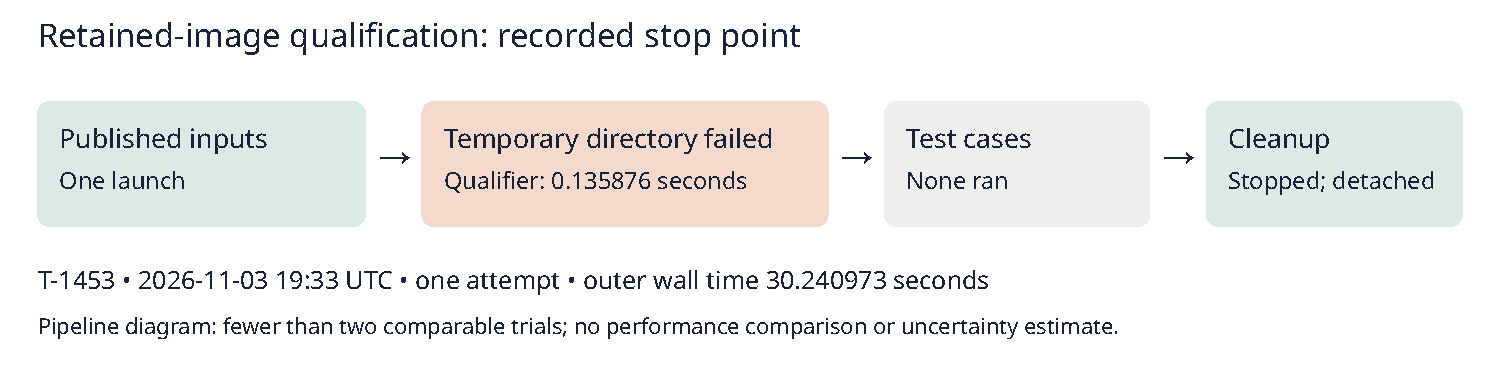
\includegraphics[width=\linewidth]{flow.pdf}

\begin{tabular}{lr}
Recorded quantity & Value\\\hline
Outer wall time (seconds) & 30.240972875\\
Service CPU time (seconds) & 6.903\\
Qualifier elapsed time (seconds) & 0.135876126\\
Test cases passed (count) & 0\\
Conservative worker debit (seconds) & 600\\
Remaining reserved campaign allowance (seconds) & 23400
\end{tabular}

\textbf{Inputs and limits.} Exact source, bindings, review and launch command were published and independently read back at GitHub commit \texttt{f4fd538dde08e293aa6895c472f18d5349f7599e}. One attempt, 300 seconds, two CPUs, 2 GiB RAM, retained 4 GiB disk. Campaign deadline: 2026-11-04 06:00 UTC. USD1 qualification allocation; total reservations USD57. Actual dollar cost is not measured. Prior costs remain recorded.

\textbf{Evidence and custody.} See parent-directory publication.json, launch.json, completion.json, native-worker-result.json, native-receipt.json, journal.stdout and qualifier-receipt.stdout. Stopped unit, absent cgroup and empty associated loop inventory were observed. The qualifier receipt was extracted using read-only debugfs under a 30-second, 512 MiB limit. Disk metadata was unchanged by extraction; no content rehash was performed during extraction. The worker's new disk digest is retained separately from the historical assembly digest.

\textbf{Scope and next step.} This is a runtime qualification result, with no scientific target execution. Diagnose temporary-directory placement within the private mount namespace; any successor needs new exact source bindings and prospective review. The flow diagram uses the recorded stop point because there is only one attempt, not comparable trial data. Source: the 26-file native-result packet manifest.
\end{document}
